\documentclass[output=paper]{langsci/langscibook} 
\author{Isabelle Udry\orcid{}\affiliation{University of Fribourg, Institut de Plurilinguisme; Zurich University of Teacher Education}}
\title[Creative thinking in task-based language teaching]
      {Creative thinking as an individual difference in task-based language teaching and learning}
\abstract{Creative thinking is an individual difference variable worth to be investigated in the context of task-based language teaching (TBLT) which requires learners to accomplish communicative tasks by using their own ideas. It is hypothesized that creative students are at an advantage in the TBLT classroom because they produce and elaborate ideas more easily and have therefore more opportunity to engage with the target language. The present chapter seeks to clarify the role of creative thinking in instructed foreign language (FL) learning for primary school children who are taught in the TBLT paradigm. The research question is whether creative thinking has an effect on a) FL proficiency and b) FL motivation. To this aim, 87 learners of L2 French and L3 English (mean age 11.1 years) completed tests on non-verbal creative thinking, crystallized intelligence, C-Tests (L2 French), reading and listening comprehension (L3 English), as well as a questionnaire on FL motivation. Data was analyzed by means of structural equation modelling. The results show an association between creative thinking and FL proficiency. No effect was found for creative thinking on FL motivation. }
\IfFileExists{../localcommands.tex}{
  \addbibresource{localbibliography.bib}
  % add all extra packages you need to load to this file

\usepackage{tabularx,multicol}
\usepackage{url}
\urlstyle{same}

\usepackage{listings}
\lstset{basicstyle=\ttfamily,tabsize=2,breaklines=true}

%\usepackage{langsci-optional}
\usepackage{langsci-lgr}
\usepackage{langsci-gb4e}
\usepackage{langsci-optional}

\usepackage{enumitem}
\usepackage[group-digits=false, detect-weight=true]{siunitx}

\usepackage{todonotes}

  \newcommand*{\orcid}{}
 
  %% hyphenation points for line breaks
%% Normally, automatic hyphenation in LaTeX is very good
%% If a word is mis-hyphenated, add it to this file
%%
%% add information to TeX file before \begin{document} with:
%% %% hyphenation points for line breaks
%% Normally, automatic hyphenation in LaTeX is very good
%% If a word is mis-hyphenated, add it to this file
%%
%% add information to TeX file before \begin{document} with:
%% %% hyphenation points for line breaks
%% Normally, automatic hyphenation in LaTeX is very good
%% If a word is mis-hyphenated, add it to this file
%%
%% add information to TeX file before \begin{document} with:
%% \include{localhyphenation}
\hyphenation{
affri-ca-te
affri-ca-tes 
Soa-res
scru-ti-ny
me-ta-cog-ni-tion
}

\hyphenation{
affri-ca-te
affri-ca-tes 
Soa-res
scru-ti-ny
me-ta-cog-ni-tion
}

\hyphenation{
affri-ca-te
affri-ca-tes 
Soa-res
scru-ti-ny
me-ta-cog-ni-tion
}
 
  \togglepaper[1]%%chapternumber
}{}

\begin{document}
\maketitle 

\section{Rationale for this chapter}\label{sec:06:1}

This chapter deals with the cognitive mechanisms underlying creativity and their impact on foreign language (FL) proficiency and motivation. Task-based language teaching (TBLT) is the common method of instruction across Switzerland. TBLT conveys language through meaningful tasks that need to be completed using the target language (\citealt{Willis1996}, \citealt{Ellis2017}; see section 2.3 for details). In the region of this study, TBLT often requires students to use language in connection with creative thinking to produce an outcome, such as a poem, a rap, or a role-play. It is reasonable to assume that creative individuals cope better with such tasks, because they are more skilled at generating and developing ideas. As a result, they may have more opportunity to engage with the target language (\citealt{Otto1998}, \citealt{Albert2006}). From a language processing perspective, creative people are assumed to be better equipped to handle basic processes, such as filtering linguistic input, dealing with novelty, and tolerating ambiguity, thus potentially progressing faster at language learning \citep{Kharkhurin2012}. 

Furthermore, creative children may simply have more fun in the TBLT classroom because they can use their imagination to be creative in their production. This may foster their enjoyment of learning a foreign language and their intrinsic motivation to do so.

In terms of classroom teaching, some authors have speculated that if creativity could enhance language learning capacity, it might be a good idea to promote creative thinking with specific programs \citep{Kharkhurin2012}. In the creative cognition rationale, such a training is deemed possible, even desirable in an educational context (\citealt{FinkeEtAl1992}, \citealt{Vogt2010}). At the same time, the needs of less creative learners would have to be considered carefully as they could be disadvantaged in a learning environment that strongly builds on creative thinking \citep{Otto1998}. Similarly, a reversed association can be assumed, i.e. that language learning has a favourable impact on creative thinking (\citealt{GhonsoolyShowqi2012}). 

\citet{DoernyeiRyan2015} suggest that creativity is a relevant ID for FL learning in current language teaching methodology. But rather than focusing on its relationship with other IDs, they argue for “paying greater attention to the interface between an individual’s inherent creativity as a predisposition and the external environment” \citep[175]{DoernyeiRyan2015}. The present study adopts this perspective by focusing on the role of children’s creative thinking in the TBLT environment with a sample of 87 children (mean age 11.1) learning L2 French and L3 English from the project Language Aptitude at Primary School (LAPS) I.

\section{Review of the literature}
\subsection{Creative thinking and foreign language learning}\label{sec:06:2.1}

Creativity covers an array of abilities that are reflected just as much in outstanding artistic performances, scientific innovation, or everyday ingenuity. The construct subsumes cognitive, motivational, personality-linked, societal and procedural aspects which have been incorporated into different theories of creativity (for an overview, see \citealt{Lubart1994}). Cognitive mechanisms underlying creativity have been described as one of the construct’s key components \citep{Lubart1994} and are thought to draw on the same cognitive structures as other intellectual abilities. Several authors have therefore integrated creativity into theories of intellect, namely \citegen{Guilford1959} Structure of intellect, \citegen{Sternberg1985} theory of successful intelligence, or \citegen{Carroll1993} model of human cognitive abilities.

The relationship between creativity and intelligence has been discussed extensively (\citealt{SternbergOHara1999}) and currently, they are considered separate, but overlapping constructs \citep{Vogt2010}. This overlap is relevant for the present study, because it can lead to an overestimation of the statistical effect of creative thinking on FL proficiency. Intelligence has therefore been included as a control variable to the statistical analysis (see \sectref{sec:06:3.3}).

As early as 1959, Guilford described two distinct but complementary creative thought processes: Divergent thinking (ability to produce and elaborate many different and/or unusual ideas) and convergent thinking (ability to select good ideas and turn them into a product). They are still at the core of creative cognition studies today, with divergent thinking being more frequently investigated \citep{Cropley2006}. This study therefore defines creative thinking as divergent thinking and the terms will be used synonymously in the remainder of the chapter.

Divergent thinking draws on memory functioning, executive control, and metacognition. More specifically, it requires an individual to cope with a new situation by retrieving existing knowledge, focusing on important information and transforming it in order to form novel associations and generate ideas to solve a problem or accomplish a task. To do this successfully, individuals must separate relevant from irrelevant information and tolerate ambiguity when an answer is not immediately available (\citealt{FinkeEtAl1992}, \citealt{Cropley2006}).

Similar processes are hypothesised to be involved in learning a foreign language. For instance, \citet{GrigorenkoEtAl2000} emphasize that successful language learners are able to deal well with novelty and tolerate ambiguity in the face of new and unfiltered linguistic material. Also, they can access existing knowledge easily and merge it with new information in order to fill linguistic gaps. People with these abilities are speculated to be at the same time creative and good language learners \citep{Kharkhurin2012}.

\subsection{Studies on creative thinking and L2 learning} 

An early study by \citet{Carroll1964} mentioned in \citet{Otto1998} identified creativity as a poor predictor for L2 proficiency. In a review of personality correlates contributing to L2 achievement, \citet{Gardner1990} even reports a negative correlation between creativity and French proficiency. The authors argue that these findings may be linked to the audiolingual method prevalent at the time of the investigation which concentrated on teaching linguistic structures, leaving little scope for creativity (\citealt{Otto1998}, \citealt{Gardner1990}). Therefore, \citet{Otto1998} readdressed the question in a more contemporary communicative teaching environment. He found significant positive correlations between creative thinking and L2 English grades in 36 Hungarian high school students. These results could not be replicated by \citet{Albert2006} who investigated the relationship between L2-proficiency, creative thinking and language aptitude in 41 advanced L2 English learners in their first year at university. The author even found negative correlations between some aspects of creative thinking (fluency and flexibility) and phonetic coding ability which is a component of language aptitude. \citet{AlbertKormos2011} revisited the issue by focusing on narration and creativity in 76 Hungarian English learners at secondary school (15--16 years). Again, they observed no significant correlation between creativity and narration complexity, accuracy and lexical diversity.

The influence of language tuition on creative thinking was examined by (\citealt{GhonsoolyShowqi2012}). They compared creative thinking in advanced English learners ($n=60$, 15--16 years) to a control group ($n=60$) of the same age that had never attended foreign language classes. Intelligence was controlled for with a non-verbal intelligence test. English learners scored significantly higher on creative thinking than the control group. In a follow up study (\citealt{ShowqiGhonsooly2015}) compared language awareness and creative thinking in beginning and advanced English learners. In both groups, significant positive correlations between the two constructs were identified. Based on their results, the authors argue that language tuition is beneficial for creative thinking.

\citet{FleithEtAl2002} examined the effects of a creativity training intervention on divergent thinking in Brazilian children who attended either a monolingual Portuguese school or a bilingual Portuguese-English program. Their aim was twofold: to assess training effects from the intervention and investigate group differences between immersion and conventional students. Treatment slightly improved divergent thinking abilities. However, divergent thinking was not related to attendance of a mono- or bilingual school program. 

Studies reported here have produced mixed findings. This may be due in part to methodological choices, i.e the fact that different age groups and aspects of language were investigated, making it difficult to compare results. 

\subsection{Creative thinking and TBLT}

Creative thinking plays a role in educational achievement, especially when knowledge is conveyed through open-ended, game like elements that incite active involvement \citep{Runco2004}. As far as foreign language learning is concerned, TBLT is a tool that can meet these criteria. Tasks can be defined as goal-oriented, meaning-focused activities which require learners to use language in order to achieve a real outcome \citep[2]{Willis1996}. In addition, tasks are meaningful, i.e. they relate to real-life, and contain some kind of a gap that needs to be filled with information or an opinion \citep{Ellis2017}. Tasks can be focused (with a communicative aim using a particular language structure), or unfocused (with a general communicative aim) \citep{Ellis2009}. 

TBLT has developed from communicative language teaching (CLT, \citealt{Krashen1981}) and, over time, a weak and strong form have emerged \citep[109]{Ellis2017}. In its strong form, TBLT aims at learning \textit{through} communication independent of curricular prescriptions \citep{Ellis2017}. Tasks guide the learning process as they provide the medium by which structural issues are raised, for instance when a specific communicative need or problem arises. The correct use of the target language is secondary.

The weak form of TBLT is found in task-supported language teaching (TSLT) which, like its \textit{strong} counterpart, primarily fosters communicative skills in the target language. Contrary to the strong form, TSLT draws on a prescribed syllabus and language is conveyed in a way that resembles the presentation-practice-production (PPP) model. In TSLT, tasks are considered an opportunity for learners to use the language they have learnt in a communicative context, usually in the production phase of the teaching cycle. In terms of vocabulary and grammar teaching, TSLT directs learner’s attention to specific linguistic forms, often explicitly in a focus-on-form element of a lesson. While communication is clearly the main objective of TSLT, the correct use of the target language is also emphasized to some extent. 

TBLT is implemented differently by teachers \citep{Ellis2009} and there is a variety of task types that draw on different learner skills and abilities \citep{Skehan1996}. For a discussion of key concepts and common misunderstandings relating to TBLT, the reader is referred to \citet{Ellis2009}.  

\subsection{TBLT in the Swiss curriculum}\label{sec:06:2.4}

As detailed in Chapter 2 this volume, the Swiss curriculum emphasizes communication in the target language and puts less importance on the correct use of form. Teaching methods in the region of this study are oriented towards CLT and more specifically a weak form of TBLT. The teaching manuals, which are prescribed by the local boards of education,\footnote{In LAPS I schools: \textit{Mille feuilles} \citep{BertschyEtAl2012} for L2 French; \textit{New World} \citep{ArnetClarkEtAl2013} for L3 English} are structured around teaching units on specific topics (e.g., sports, art, or storytelling) which are introduced to learners via authentic written or auditory input. The authentic input is consolidated with a series of meaning-based activities that prepare pupils for the communicative task at the end of each unit. In the process, pupils are made familiar with some predetermined aspects of grammar and vocabulary. 

The teaching manuals highlight the use of creative thinking in the communicative task where learners need to draw on the target language to plan and elaborate a creative product. For instance, children design a poster about a particular sport, create a piece of artwork and describe it to their peers at a vernissage, or turn a short story into a play that is presented to the class \citep{ArnetClarkEtAl2013}. Group presentations are followed up with a personal reflection on the task process. ‘Project tasks’, as they are called in the L3 English manual \citep{ArnetClarkEtAl2013}, are carried out individually or in groups. The hypothesized link with creative thinking outlined in section 2.1 is particularly evident in this type of TBLT scenario. Individual differences in creative thinking are therefore expected to affect task performance and consequently language proficiency. 

\subsection{Creative thinking and FL motivation}

FL motivation and related constructs are discussed in Chapter 1, \sectref{sec:01:3}. The link between creative thinking and FL motivation in the TBLT classroom is underpinned by \citeauthor{DeciRyan1985}'s (\citeyear{DeciRyan1985,DeciRyan2002}) self-determination theory (SDT). A key concept of SDT is intrinsic motivation, i.e. an inherent drive to engage with the environment that is largely independent of external sources. Intrinsic motivation resides on three basic individual needs: self-determination, competence, and interpersonal relatedness. I argue that TBLT with a focus on creative thinking can meet these needs in several ways: giving children the opportunity to elaborate on their own ideas contributes to their feeling autonomous and competent. Working with others and getting feedback on their outcomes strengthens a sense of competence and connectedness to the group.

The opportunity to be creative while studying a language is expected to affect enjoyment of learning and therefore intrinsic FL motivation. Forms of extrinsic motivation, such as wanting to earn good grades or keep up with other students, are deemed less relevant for this context and are not considered in the analysis. In what follows, \textit{French motivation} and \textit{English motivation} therefore refers to intrinsic motivation only. 

In terms of the structure of FL motivation as assessed in our student questionnaire, the factor analysis reported in Chapter 3 points to two different factors: Intrinsic motivation, L2 self-concept, and L2 anxiety form a common factor we call \textit{L2 Academic Emotion}. Extrinsic items, dedication, and teacher/parental support load onto a separate factor we refer to as \textit{Extrinsic Factor}. Regression analysis shows a substantial contribution of L2 Academic Emotion to L2 proficiency, while the extrinsic factor is not associated positively with L2 proficiency.

\section{Method}
\subsection{Research questions}

Two research questions are addressed in this chapter:

\begin{enumerate} 

\item What is the association between creative (divergent) thinking and FL proficiency? 

Based on current research findings and theoretical arguments on creative cognition and TBLT, it is hypothesized that creative thinking (assessed in a non-verbal test for divergent thinking) is positively related to children’s FL proficiency. Learners with well-developed creative thinking skills are expected to be at an advantage in TBLT due to an enhanced ability to generate and elaborate ideas. It is assumed that they have more capacity to invest in actual language work, thus progressing faster at language learning.

\item Does creative thinking relate to students’ intrinsic FL motivation in the TBLT classroom? 

To the author’s knowledge, this question has not been studied explicitly yet. Considering aspects of TBLT outlined in section 2.3 and theories of FL motivation discussed in Chapter 1, a positive association between creative thinking and intrinsic motivation to learn in the TBLT classroom is hypothesized. TBLT is thought to enhance creative children’s enjoyment of FL learning because particular attention is given to their ideas. 
\end{enumerate}

\subsection{Participants and procedure}

The research design of the LAPS project is described in Chapter 2, and only aspects relevant to this study are summarized here.

The sample has been derived from LAPS I and included a total of 117 5\textsuperscript{th} graders (mean age 11.1 years in spring 2017) learning L2 French and L3 English. Children with L1 English or L1 French, as well as incomplete observations were excluded from the sample, leaving 87 complete observations for data analysis.

At T1 (spring 2017), creative thinking, intelligence, and L2 French were tested and children filled in a L2 French motivation questionnaire. A L2/L3 motivation questionnaire and L3 English test were administered a year later at T2. At the time of testing, participants had received 248 French lessons over 2.5 academic years (T1) and 152 English lessons over 1.5 academic years (T2). 

Creativity was operationalized as divergent creative thinking and assessed with the Test of Creative Thinking (Divergent Production) (TCT-DP) by \citet{UrbanJellen1995}. Participants need to complete an unfinished picture with 6 figural fragments presented to them on paper. There is no time constraint and participants are told that they are free to draw whatever they like. The test is scored according to 14 criteria (see Chapter 2, \sectref{sec:02:3}). This non-verbal test was chosen in order to rule out language as a confounding variable \citep{Simonton2008}.

Intelligence was measured with the number sequencing subtest of the CFT 20-R \citep{Weiss2006} for crystallized intelligence. 

L2 French was assessed with a C-Test composed of four short and independent paragraphs \citep{Grotjahn2002}. L3 English was measured with the Oxford young learners’ placement test OYLPT (\citealt{Testing2013}). It covers reading and listening comprehension. The test assesses language use, vocabulary, and grammar embedded in everyday situations. Due to the overall aims of the project, different skills were measured at different times (see Chapter 2 for details).

The motivational questionnaire is also detailed in Chapter 2. It covers various aspects, including intrinsic and extrinsic motivation, L2/L3 self-concept, L2/L3 anxiety, dedication, and perceived encouragement by teachers and parents. For reasons discussed in \sectref{sec:06:2.4}, \textit{French motivation} and \textit{English motivation} exclusively refers to items assessing intrinsic motivation. 

\subsection{Analysis}\label{sec:06:3.3}

This Chapter explores creative thinking in two ways: In relation to FL proficiency and intrinsic FL motivation. As outlined in \sectref{sec:06:2.1}, the literature postulates an overlap between intelligence and creative thinking. The two constructs may share some of the explained variance in the statistical model, leading to biased parameter estimates (overestimation of creative thinking effects). This can be accounted for by treating intelligence as a confounder and controlling for it in the analysis \citep{Rohrer2018}. As one of the reviewers pointed out, the assumed overlap may be more related to fluid, rather than crystallized intelligence and it may have been more revealing to administer a test of fluid intelligence. Due to the overall design of the project, however, this was not possible in LAPS I (see Chapter 2 for details).

Like all psychometric constructs, intelligence (and creativity for that matter) cannot be observed directly but only measured approximately by a psychometric test. When controlling for intelligence, we actually control for the observation of the construct expressed in the individual test score. The more precise this measure, the more accurate the estimates from the statistical model will be \citep{Vanhove2015}. However, test scores are always obtained with some measurement error owed to test conditions or to the test instrument. Accounting for this measurement error in the statistical model will increase its accuracy (\citealt{BrunnerAustin2009}). As suggested by \citet{WestfallYarkoni2016}, measurement error can be accounted for by calculating the error variance of a given variable based on the reliability coefficient of its test and including the error variance in the statistical model. When addressing construct-related issues, such as the ones in this chapter, the authors recommend using structural equation modelling (SEM) or other latent-variable approaches which allow for introducing measurement error directly to the statistical model. SEM refers to a group of statistical techniques that are commonly used in social sciences to investigate unobservable latent constructs, such as creativity or intelligence. In the structural equation model, these latent constructs are represented by one or more observed variables, i.e. the instruments that assess the unobservable construct. The relationship between the latent constructs can then be estimated with independent regression equations. 

\section{Results}
\subsection{Creative thinking and FL proficiency}

Based on the arguments outlined in \sectref{sec:06:3.3}, SEM was used with the lavaan package for R \citep{Rosseel2012} to allow for a) investigation of latent constructs and b) consideration of measurement error to increase model accuracy. 

For the first research question, FL proficiency (L2 French and L3 English) was introduced to the model as an endogenous (or outcome) variable. Based on the assumption of an underlying aptitude for foreign language learning, the two languages were treated as one latent variable. The choice is further based on the multicompetence framework which hypothesizes the integration of all languages known to the learner in a common linguistic repertoire (for a recent discussion see \citealt{Cook2012}). Creative thinking (TCT-DP) and intelligence (number sequencing CFT-20 R) were introduced to the model as exogenous (or predictor) variables.

In \figref{fig:06:1}, circles show latent variables (or constructs) and squares show measured variables. One headed arrows indicate the regression coefficients or parameter estimates, i.e. the strength of association between the variables. Double headed arrows stand for variances.

\begin{figure}
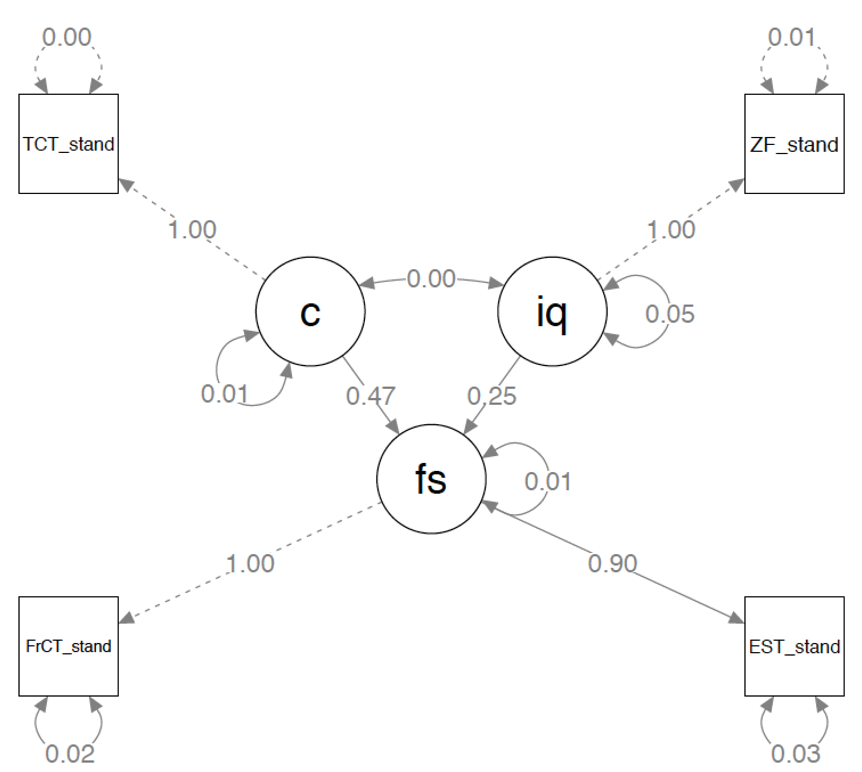
\includegraphics[width=\textwidth]{figures/Figure6.1.png}
\caption{\label{fig:06:1}Path diagram for Model 3 (reliability 0.78). Nodes (latent constructs): fs\,=\,foreign language proficiency, c\,=\,creative thinking, iq\,=\,intelligence; \mbox{TCT\_stand}\,=\,test on divergent thinking, \mbox{ZF\_stand}\,=\,number sequencing test, \mbox{FrCT\_stand}\,=\,French C-Test, \mbox{EST\_stand}\,=\,English OYLPT score.}
\end{figure}

In order to determine measurement error, the reliability coefficients for the exogenous (predictor) variables (creative thinking, intelligence) were taken from the test manuals to calculate error variances (\tabref{tab:06:1}). The obtained error variances were added to the different statistical Models 1--3. 

For the number sequencing test, a reliability coefficient of Cronbach's $\alpha$ 0.91 is reported \citep{Weiss2006}. For the TCT-DP, different values are given, ranging from 0.38 to 0.78, depending on the validation study \citep{UrbanJellen1995}. Based on recommendations by \citet{WestfallYarkoni2016}, I accounted for the TCT-DP variation by fitting three models assuming reliability coefficients of 0.38 (Model 1), 0.58 (Model 2) and 0.78 (Model 3). For ease of reading, only Model 3 will be reported in the following. Further information on all models can be found at \url{https://osf.io/vxr9m/}. 

\begin{table}
\caption{\label{tab:06:1}Exogenous (predictor) variables and their sample variance (Var), standard deviation (SD), reported reliability coefficients (RC) and calculated measurement error/error variance (ME) for this sample.}
\begin{tabular}{l cccc} 
\lsptoprule
Model 3 & {Var} & {SD} & {RC} & {ME} \\\midrule
Creative thinking (divergent thinking)      & 0.01 & 0.12 & 0.78 & 0.003\\
Intelligence (number sequencing)         & 0.06 & 0.25 & 0.91 & 0.006\\
\lspbottomrule
\end{tabular}
\end{table}

Model 3 produced acceptable fit indices\footnote{Cut off for good fit: $\text{CFI} > 0.9; \text{RMSEA} < 0.08, \text{SRMR} < 0.08$ \citep{Kline2011}.} ($\text{CFI} = 1, \text{RMSEA} = 0, \text{SRMR} = 0.01$). As shown in \tabref{tab:06:2} and \figref{fig:06:1}, Model 3 supports an effect for creative thinking on language proficiency when intelligence is controlled for in the range of statistical significance. Confidence intervals indicate some uncertainty in the parameter estimate. This result does not necessarily point to a direct causal influence from creative thinking to FL proficiency. The design used in this study does not allow for making claims on causality. 

\begin{table}
\caption{\label{tab:06:2}Estimates for Model 3 (0.78) on the association between creative thinking and intelligence and FL proficiency.}
\begin{tabular}{l SS SS SS}
\lsptoprule
{L2/L3 proficiency {\textasciitilde}} & {Est.} & {SE} & {$z$} & {$p$} & {ci lower} & {ci upper}\\\midrule
Creative thinking & 0.47 & 0.19 & 2.47 & 0.013 & 0.1 & 0.84\\
Intelligence      & 0.25 & 0.08 & 3.1 & 0.002 & 0.09 & 0.41\\
\lspbottomrule
\end{tabular}
\end{table}
\subsection{Creative thinking and FL motivation}

The opportunity to be creative in the classroom is assumed to impact particularly on intrinsic FL motivation, rather than extrinsic motivation. The SEM for the second research question therefore includes intrinsic motivation for English and French as the endogenous (outcome) variable and creative thinking as the exogenous (predictor) variable. Different models with combinations of motivation items were fitted. A total of four items were retained in the final Model 4 represented in \figref{fig:06:2} (the same symbols apply as in \figref{fig:06:1}). Combinations of other FL motivation items fitted the data less well and were therefore not pursued further.\footnote{\citet{KolenikovBollen2016} describe several possible causes for unusual model indications, referred to as Heywood cases: Outliers, empirical underidentification, structural misspecification, missing data or sampling fluctuations. The authors also give an overview of how to address these issues.} 

  
\begin{figure}
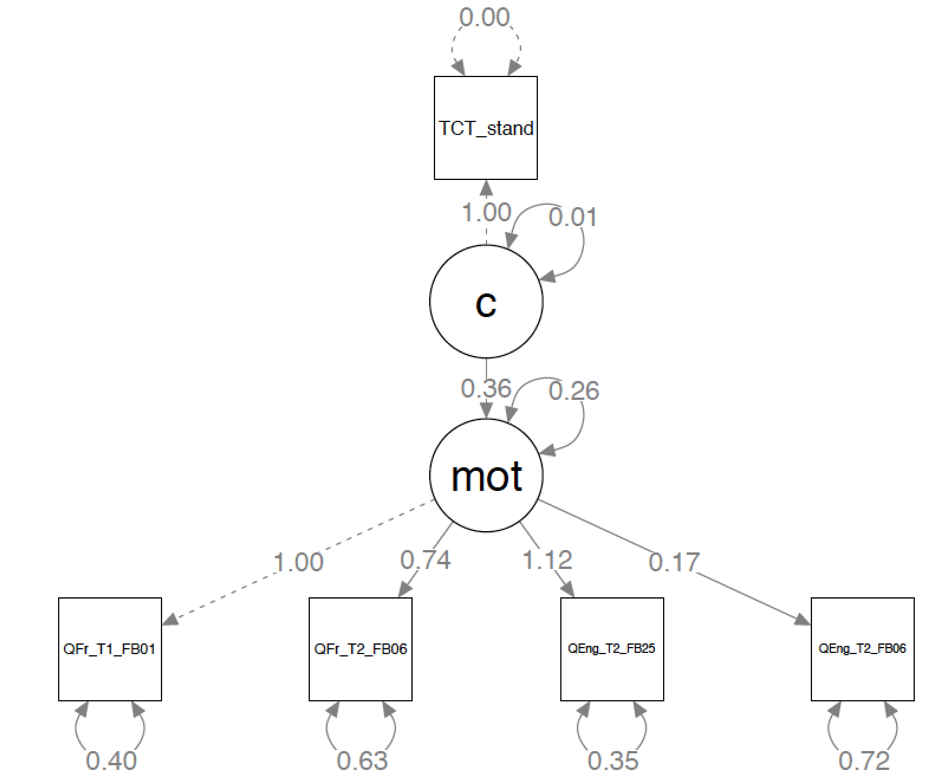
\includegraphics[width=\textwidth]{figures/Figure6.2.png}
\caption{\label{fig:06:2}Path diagram for Model 4 (reliability 0.78). Nodes: c\,=\,creative thinking, mot\,=\,intrinsic motivation (latent constructs); TCT1\,=\,test on divergent thinking, intrinsic motivation French: \mbox{QFr\_T1\_FB01}, \mbox{QFr\_T2\_FB06}, intrinsic motivation English: \mbox{QEng\_T2\_FB25\_QEng\_T2\_FB06}.}
\end{figure}

Again, different measurement errors were considered for the creative thinking test in Model 4, all options yielded the same acceptable fit to the data ($\text{CFI}=1, \text{SRMR}= 0.04, \text{RMSR}=0$). The association between creative thinking turns out to be negligible and non-significant, as indicated by the low $z$-value and high $p$-value reported in \tabref{tab:06:3}.   

\begin{table}
\caption{\label{tab:06:3}Estimates from Model 4 (0.78) on the association between motivation to learn a foreign language and creative thinking.}
\begin{tabular}{l cccccc} 
\lsptoprule
{Intrinsic Motivation {\textasciitilde}} & {Est.} & {SE} & {$z$} & {$p$} & {ci lower} & {ci upper}\\\midrule
Creative thinking & 0.36 & 0.74 & 0.49 & 0.63 & $-1.1$ & 1.81\\
\lspbottomrule
\end{tabular}
\end{table}

\section{Discussion}

Research question 1 addressed the association between creative (divergent) thinking and FL proficiency. A statistically significant effect emerges from the data, indicating that creative thinking plays a role in children’s developing FL proficiency when they are taught in the TBLT paradigm. The present study thus mirrors findings from \citet{Otto1998} with high school students and contradicts \citet{Albert2006} and \citet{AlbertKormos2011} who could not replicate results from the Ottó study. Research question 2 explored the possibility that creative children are motivated to learn foreign languages with TBLT, i.e. that high scores in the creative thinking test are associated with high values on the motivation-questionnaire items. This hypothesis could not be substantiated: the association between creative thinking and FL motivation in this sample is negligible and non-significant. 

It is worth pointing out that the results reported here do not allow for stipulating any causal links between the investigated constructs. While an effect of creative thinking on FL proficiency has been found in the data, the direction of causality remains unclear. It may well be, as some scholars suggest, that language learning contributes to creative thinking. Such claims have been made mainly with reference to simultaneous bilingualism (for an overview, see \citealt{Ricciardelli1992}), rather than exposure to instructed language learning. To address causality, \citet{Simonton2008} suggests a longitudinal design with multiple assessment of the variables where time would allow for comparison within and between subjects. If multilingualism resulting from instructed language learning were a predictor for creative thinking, this would be detected in the data if an individual’s FL proficiency at T1 and creative thinking at T2 were more strongly correlated than creative thinking at T1 and individual FL proficiency at T2 \citep[154]{Simonton2008}. However, this kind of research is rare and obviously the research design presented in this chapter does not allow for such inferences.

Some changes to the design could have improved the robustness of the findings. For instance, children’s motivation to learn foreign languages did not include questions on how they liked the teaching methods or textbooks. Also, assessing creative thinking more comprehensively, including a range of tests and information on creative hobbies might have provided a more detailed view of the creative student than a mere non-verbal test. These aspects may be considered in future studies to provide further insights into the role of creative thinking in instructed language learning. 

{\sloppy\printbibliography[heading=subbibliography,notkeyword=this]}
\end{document}
